\documentclass{article}
\usepackage{graphicx}
\graphicspath{ {Images/} }


\begin{document}
\title{Common Architectural Patterns}
\author{Yasser Ahmed Elmancy}
\date{\today}
\maketitle

\tableofcontents
\newpage

\section{Model-View-Controller}

Model View Controller or MVC as it is popularly called, is a software design pattern for developing web applications. A Model View Controller pattern is made up of the following three parts:

\begin{itemize}

\item Model - The lowest level of the pattern which is responsible for maintaining data.
\item View - This is responsible for displaying all or a portion of the data to the user.
\item Controller - Software Code that controls the interactions between the Model and View.

\end{itemize}

\noindent MVC is popular as it isolates the application logic from the user interface layer and supports separation of concerns. Here the Controller receives all requests for the application and then works with the Model to prepare any data needed by the View. The View then uses the data prepared by the Controller to generate a final presentable response. The MVC abstraction can be graphically represented in figure \ref{fig_mvc}.\\\\

\begin{figure}[h]
\centering
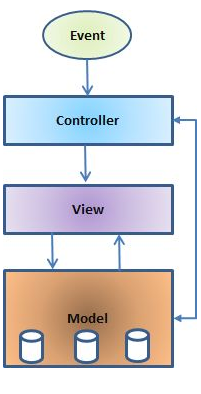
\includegraphics[scale=0.8]{mvc.png}
\caption{MVC Architecture.}
\label{fig_mvc}
\end{figure}



\section{Presentation-Abstraction-Control}

This architecture is a further development of the Model-View-Controller architecture. The MVC is restricted to simple GUI's with one or more views on the same model. If the model consists of substructures that all require they own special way of interaction, a more complex GUI architecture is in order. The PAC architecture does not have the model as its core component, but a hierarchical structure of PAC components. Each PAC component consists of these items:

\begin{itemize}

\item Presentation - It is exactly like the View of MVC. It displays the information from the Abstraction.
\item Abstraction - It contains the data, like in MVC. However, it may be just part of the complete data structure of the application, and it does not play an active role in the notification of changes.
\item Control - This is somewhat similar to the Controller in the MVC architecture. It processes external events and updates the model. It also directly updates the Presentation part. Yet it is different from the C in MVC in that it passes the changes being made to its parent PAC component.



\end{itemize}

\begin{figure}[h]
\centering
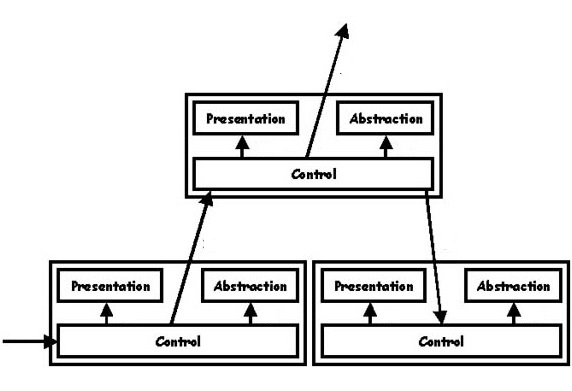
\includegraphics[scale=0.65]{pac.jpg}
\caption{PAC components are connected in a hierarchical fashion.}
\label{fig_pac}
\end{figure}



\section{Pipe And Filter}
A very simple, yet powerful architecture, that is also very robust. It consists of any number of components (filters) that transform or filter data, before passing it on via connectors (pipes) to other components. The filters are all working at the same time. The architecture is often used as a simple sequence, but it may also be used for very complex structures.

\noindent Components of this architecture are:
\begin{itemize}

\item Pump - or producer is the data source. It can be a static text file, or a keyboard input device, continuously creating new data, or data of another application.
\item Pipe - is the connector that passes data from one filter to the next. It is a directional stream of data that is usually implemented by a data buffer to store all data, until the next filter has time to process it.
\item Filter - transforms or filters the data it receives via the pipes with which it is connected. A filter can have any number of input pipes and any number of output pipes.
\item Sink - or consumer is the data target. It can be another file, a database, computer screen, or another application.\\\\

\end{itemize}

\begin{figure}[h]
\centering
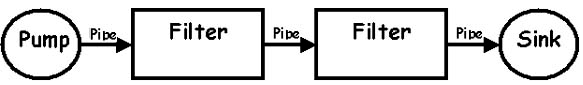
\includegraphics[scale=0.65]{p&f.png}
\caption{Pipe and filter Architecture.}
\label{fig_p&f}
\end{figure}


\newpage

\section{Layered Systems}
Layered Systems use layers to separate different units of functionality. Each layer only communicates with the layer above and the layer below. Each layer uses the layer below to perform its function. Communication happens through predefined, fixed interfaces. A Layer is a design construct. It is implemented by any number of classes or modules that behave like they are all in the same layer. That means that they only communicate with classes in layers immediately above or below their layer and with themselves. Each layer offers its own kind of functionality. A higher layer uses its lower layer to perform its function. It requires its lower layer. It is possible to define multiple layers at the same level. The user calls a function on an object in the upper layer. This object calls functions in the layer below. These functions in turn approach the layer below and the layer above.

\noindent There are five architectural patterns for layered systems that will be discussed later:
\begin{itemize}

\item Master-slave architecture.
\item Two-tier client–server architecture.
\item Multi-tier client–server architecture.
\item Distributed component architecture.
\item Peer-to-peer architecture

\end{itemize}

\begin{figure}[h]
\centering
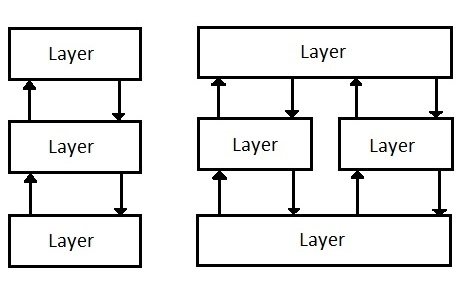
\includegraphics[scale=0.65]{ls.jpg}
\caption{Layered Systems Architecture.}
\label{fig_ls}
\end{figure}



\section{Microkernal}
The microkernel architecture pattern consists of two types of architecture components: a core system and plug-in modules. Application logic is divided between independent plug-in modules and the basic core system, providing extensibility, flexibility, and isolation of application features and custom processing logic. Figure \ref{fig_mk} illustrates the basic microkernel architecture pattern.\\\\

\begin{figure}[h]
\centering
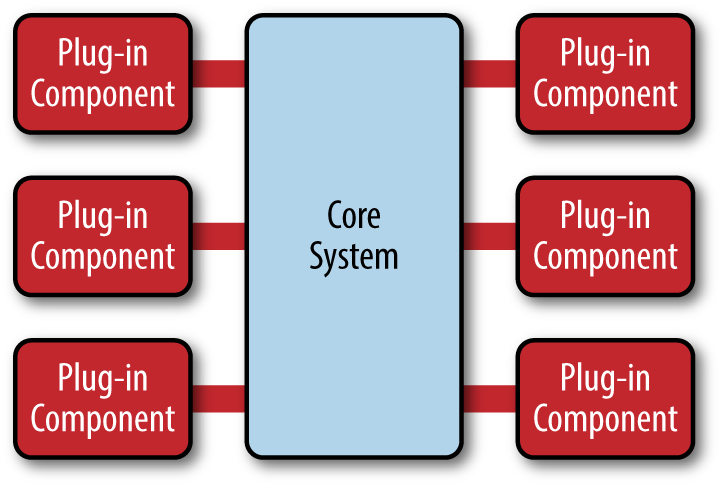
\includegraphics[scale=1.7]{mk.png}
\caption{Microkernal Architecture.}
\label{fig_mk}
\end{figure}

\noindent The core system of the microkernel architecture pattern traditionally contains only the minimal functionality required to make the system operational. Many operating systems implement the microkernel architecture pattern, hence the origin of this pattern's name. From a business-application perspective, the core system is often defined as the general business logic sans custom code for special cases, special rules, or complex conditional processing.
\newpage


\section{Client-Server}
A Client-Server Architecture consists of two types of components: clients and servers. A server component perpetually listens for requests from client components. When a request is received, the server processes the request, and then sends a response back to the client. Servers may be further classified as stateless or stateful. Clients of a stateful server may make composite requests that consist of multiple atomic requests. This enables a more conversational or transactional interactions between client and server. To accomplish this, a stateful server keeps a record of the requests from each current client. This record is called a session.\\\\

\begin{figure}[h]
\centering
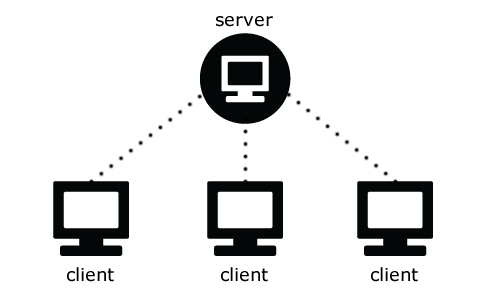
\includegraphics[scale=1]{client-server.png}
\caption{Client-Server Architecture.}
\label{fig_cs}
\end{figure}

\newpage

\section{N-Tier}
N-Tier architecture is a Client-Server architecture combined with the Layered architecture where N equals three or higher. Three-Tier architecture is an example of N-Tier architecture. It consists of:

\begin{itemize}

\item Presentation Layer - deals with user interactions. Thin clients interface do not contain business logic, just code required to process user input, send requests to the server, and show the results of these requests. 
\item Application Layer - It is the actual web application that performs all functionality specific to the web application. However, it does not store the persistent data itself. Whenever it needs data of any importance, it contacts the DB server. 
\item Database Layer - contains Database and Database Management System. 

\end{itemize}


\begin{figure}[h]
\centering
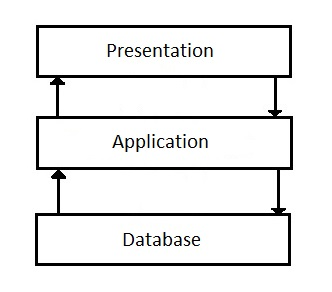
\includegraphics[scale=1]{3t.jpg}
\caption{Three-Tier Architecture.}
\label{fig_3t}
\end{figure}

\newpage
\noindent Another example is Four-Tier architecture which consists of:

\begin{itemize}

\item Presentation Layer - It is concerned with presenting information to the user and managing all user interaction.
\item Data Management Layer - Manages the data that is passed to and from the client. This layer may implement checks on the data, generate web pages, etc.
\item Application Processing Layer - It is concerned with implementing the logic of the application and so providing the required functionality to end users.
\item Database Layer - Stores the data and provides transaction management services, etc.

\end{itemize}

\begin{figure}[h]
\centering
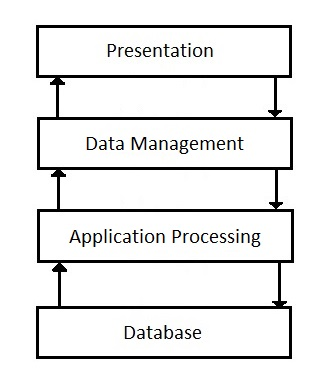
\includegraphics[scale=0.9]{4t.jpg}
\caption{Four-Tier Architecture.}
\label{fig_4t}
\end{figure}

\section{Repository}
The Repository Pattern is one of the most popular patterns to create an enterprise level application. It restricts us to work directly with the data in the application and creates new layers for database operations, business logic and the application UI. If an application does not follow the Repository Pattern, it may have the following problems:

\begin{itemize}

\item Duplicate database operations codes.
\item Need of UI to unit test database operations and business logic.
\item Need of External dependencies to unit test business logic.

\end{itemize}

\noindent Using the Repository Pattern has many advantages:
\begin{itemize}

\item Your business logic can be unit tested without data access logic.
\item The database access code can be reused.
\item Your database access code is centrally managed so easy to implement any database access policies, like caching.

\end{itemize}

\begin{figure}[h]
\centering
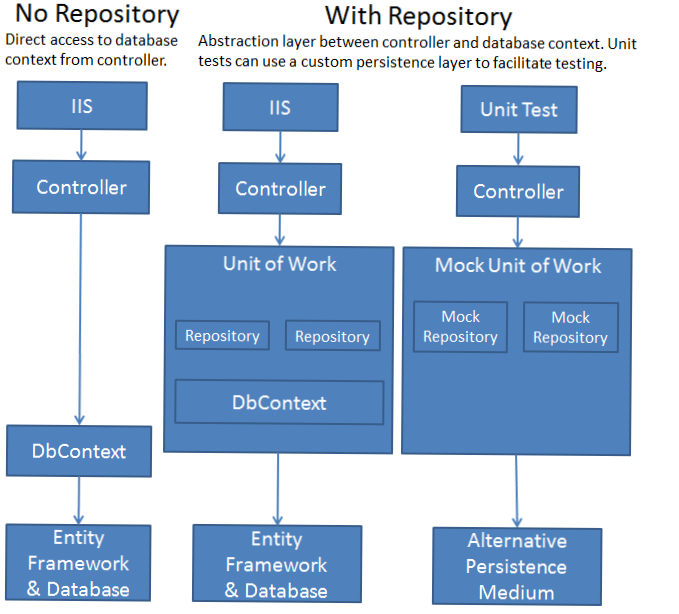
\includegraphics[scale=0.55]{r.png}
\caption{With or without repository Architecture.}
\label{fig_r}
\end{figure}
	


\section{Blackboard}
The Blackboard pattern shows how a complex problem, such as image or speech recognition can be broken up into smaller, specialized subsystems that work together to solve a problem. It is useful for problems for which no deterministic solution strategies are known. In blackboard, several specialized subsystems assemble their knowledge to build a possibly partial or approximate solution.\\
The blackboard pattern consists of three components:

\begin{itemize}

\item Blackboard
\begin{itemize}
\item Central data storage.
\item Acts as an interface for knowledge-sources to read or write to it.
\end{itemize}

\item Knowledge-sources
\begin{itemize}
\item Independent sub-systems which exists separately.
\item Provides solution to some part of entire problem.
\item Results of all KS are integrated to solve the entire problem.
\end{itemize}

\item Control
\begin{itemize}
\item Monitor changes on blackboard periodically (run a loop).
\item On identifying changes, decide the action to take place.
\item Schedule knowledge-source execution.
\end{itemize}

\end{itemize}

\begin{figure}[h]
\centering
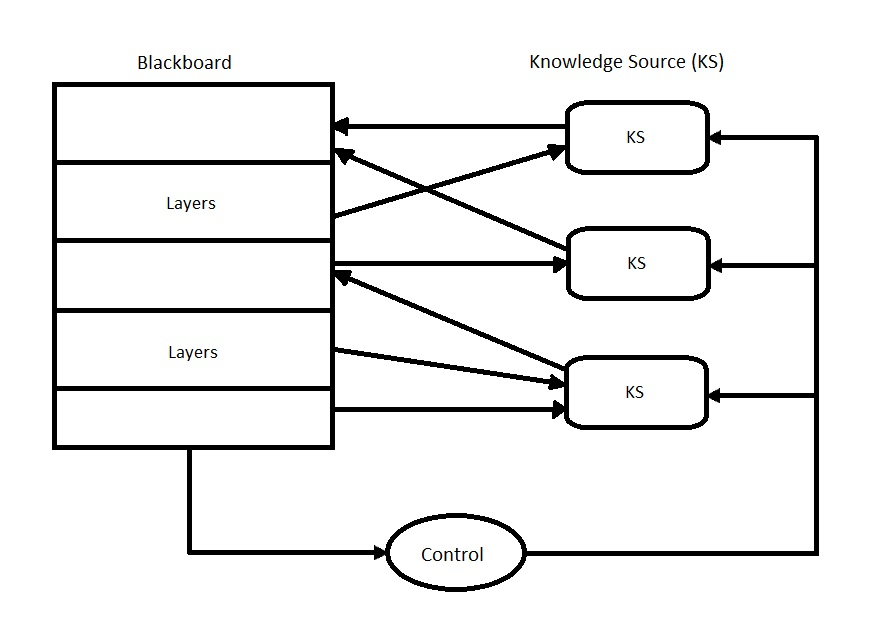
\includegraphics[scale=0.3]{bb.jpg}
\caption{Blackboard Architecture.}
\label{fig_bb}
\end{figure}
	


\section{Finite State Machine}
In general, a state machine is any device that stores the status of something at a given time and can operate on input to change the status and/or cause an action or output to take place for any given change. A computer is basically a state machine and each machine instruction is input that changes one or more states and may cause other actions to take place. Each computer's data register stores a state. The read-only memory from which a boot program is loaded stores a state (the boot program itself is an initial state). The operating system is itself a state and each application that runs begins with some initial state that may change as it begins to handle input. Thus, at any moment in time, a computer system can be seen as a very complex set of states and each program in it as a state machine. In practice, however, state machines are used to develop and describe specific device or program interactions.\\\\


\noindent To summarize it, a state machine can be described as:
\begin{itemize}

\item An initial state or record of something stored someplace.
\item A set of possible input events.
\item A set of new states that may result from the input.
\item A set of possible actions or output events that result from a new state.\\\\

\end{itemize}

\noindent A finite state machine is one that has a limited or finite number of possible states. (An infinite state machine can be conceived but is not practical.) A finite state machine can be used both as a development tool for approaching and solving problems and as a formal way of describing the solution for later developers and system maintainers.

\newpage


\section{Process Control}
Real time dynamic control systems are used to allow digital systems to interact with the physical world, for example: control systems for machines and engines. Such systems use sensors to receive information, perform computations, and control the machine or engine via actuators. Unlike applications based on iterative refinement, real time control systems are designed with the intention for the control process to continue indefinitely.\\

\noindent For example, an engine control unit receives the accelerator's position and current RPM as inputs, and changes the amount of fuel injected into the cylinders so that the amount of torque produced by such engine corresponds to the accelerator's position.\\

\noindent Frequently these systems take the form of a dynamic, stateful system which provides sensor feedback to a controller. The controller then has access to a set of parameters that modify the dynamics of the system. The system under control is usually stochastic and unpredictable, and has real-time constraints; correct functionality depends upon deadline-driven response to sensor feedback. Engines and machines generate analog information. Digital Control Theory was developed so that micro-controllers and computers could be used to perform such control tasks.\\\\


\begin{figure}[h]
\centering
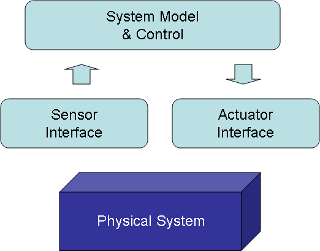
\includegraphics[scale=0.8]{pc.png}
\caption{Process control model.}
\label{fig_pc}
\end{figure}
	



\section{Multi Agent System}
A multi-agent system (M.A.S.) is a computerized system composed of multiple interacting intelligent agents within an environment. Multi-agent systems can be used to solve problems that are difficult or impossible for an individual agent or a monolithic system to solve. Intelligence may include some methodic, functional, procedural approach, algorithmic search or reinforcement learning. Although there is considerable overlap, a multi-agent system is not always the same as an agent-based model (ABM). The goal of an ABM is to search for explanatory insight into the collective behavior of agents (which don't necessarily need to be "intelligent") obeying simple rules, typically in natural systems, rather than in solving specific practical or engineering problems. The terminology of ABM tends to be used more often in the sciences, and MAS in engineering and technology.\\\\



\begin{figure}[h]
\centering
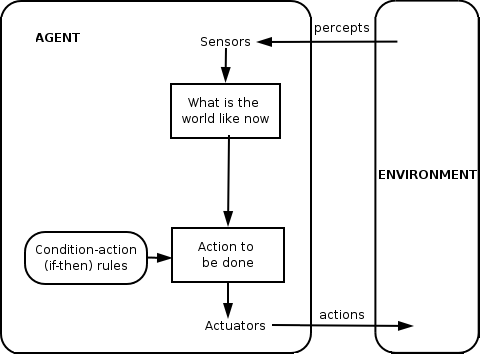
\includegraphics[scale=0.7]{mas.png}
\caption{Simple reflex agent.}
\label{fig_mas}
\end{figure}

\newpage	


\section{SOA}
A service-oriented architecture (SOA) is a style services are provided to the other components by application components, through a communication protocol over a network. The basic principles of SOA are independent of vendors, products and technologies. A service is a discrete unit of functionality that can be accessed remotely and acted upon and updated independently, such as retrieving a credit card statement online.\\

\noindent A service has four properties according to one of many definitions of SOA:
\begin{itemize}

\item It logically represents a business activity with a specified outcome.
\item It is self-contained.
\item It is a black box for its consumers.
\item It may consist of other underlying services.\\

\end{itemize}
Different services can be used in conjunction to provide the functionality of a large software application. Service-oriented architecture is more about how to compose an application by integration of distributed, separately-maintained and deployed software components. It is enabled by technologies and standards that make it easier for components to communicate and cooperate over a network.\\\\



\begin{figure}[h]
\centering
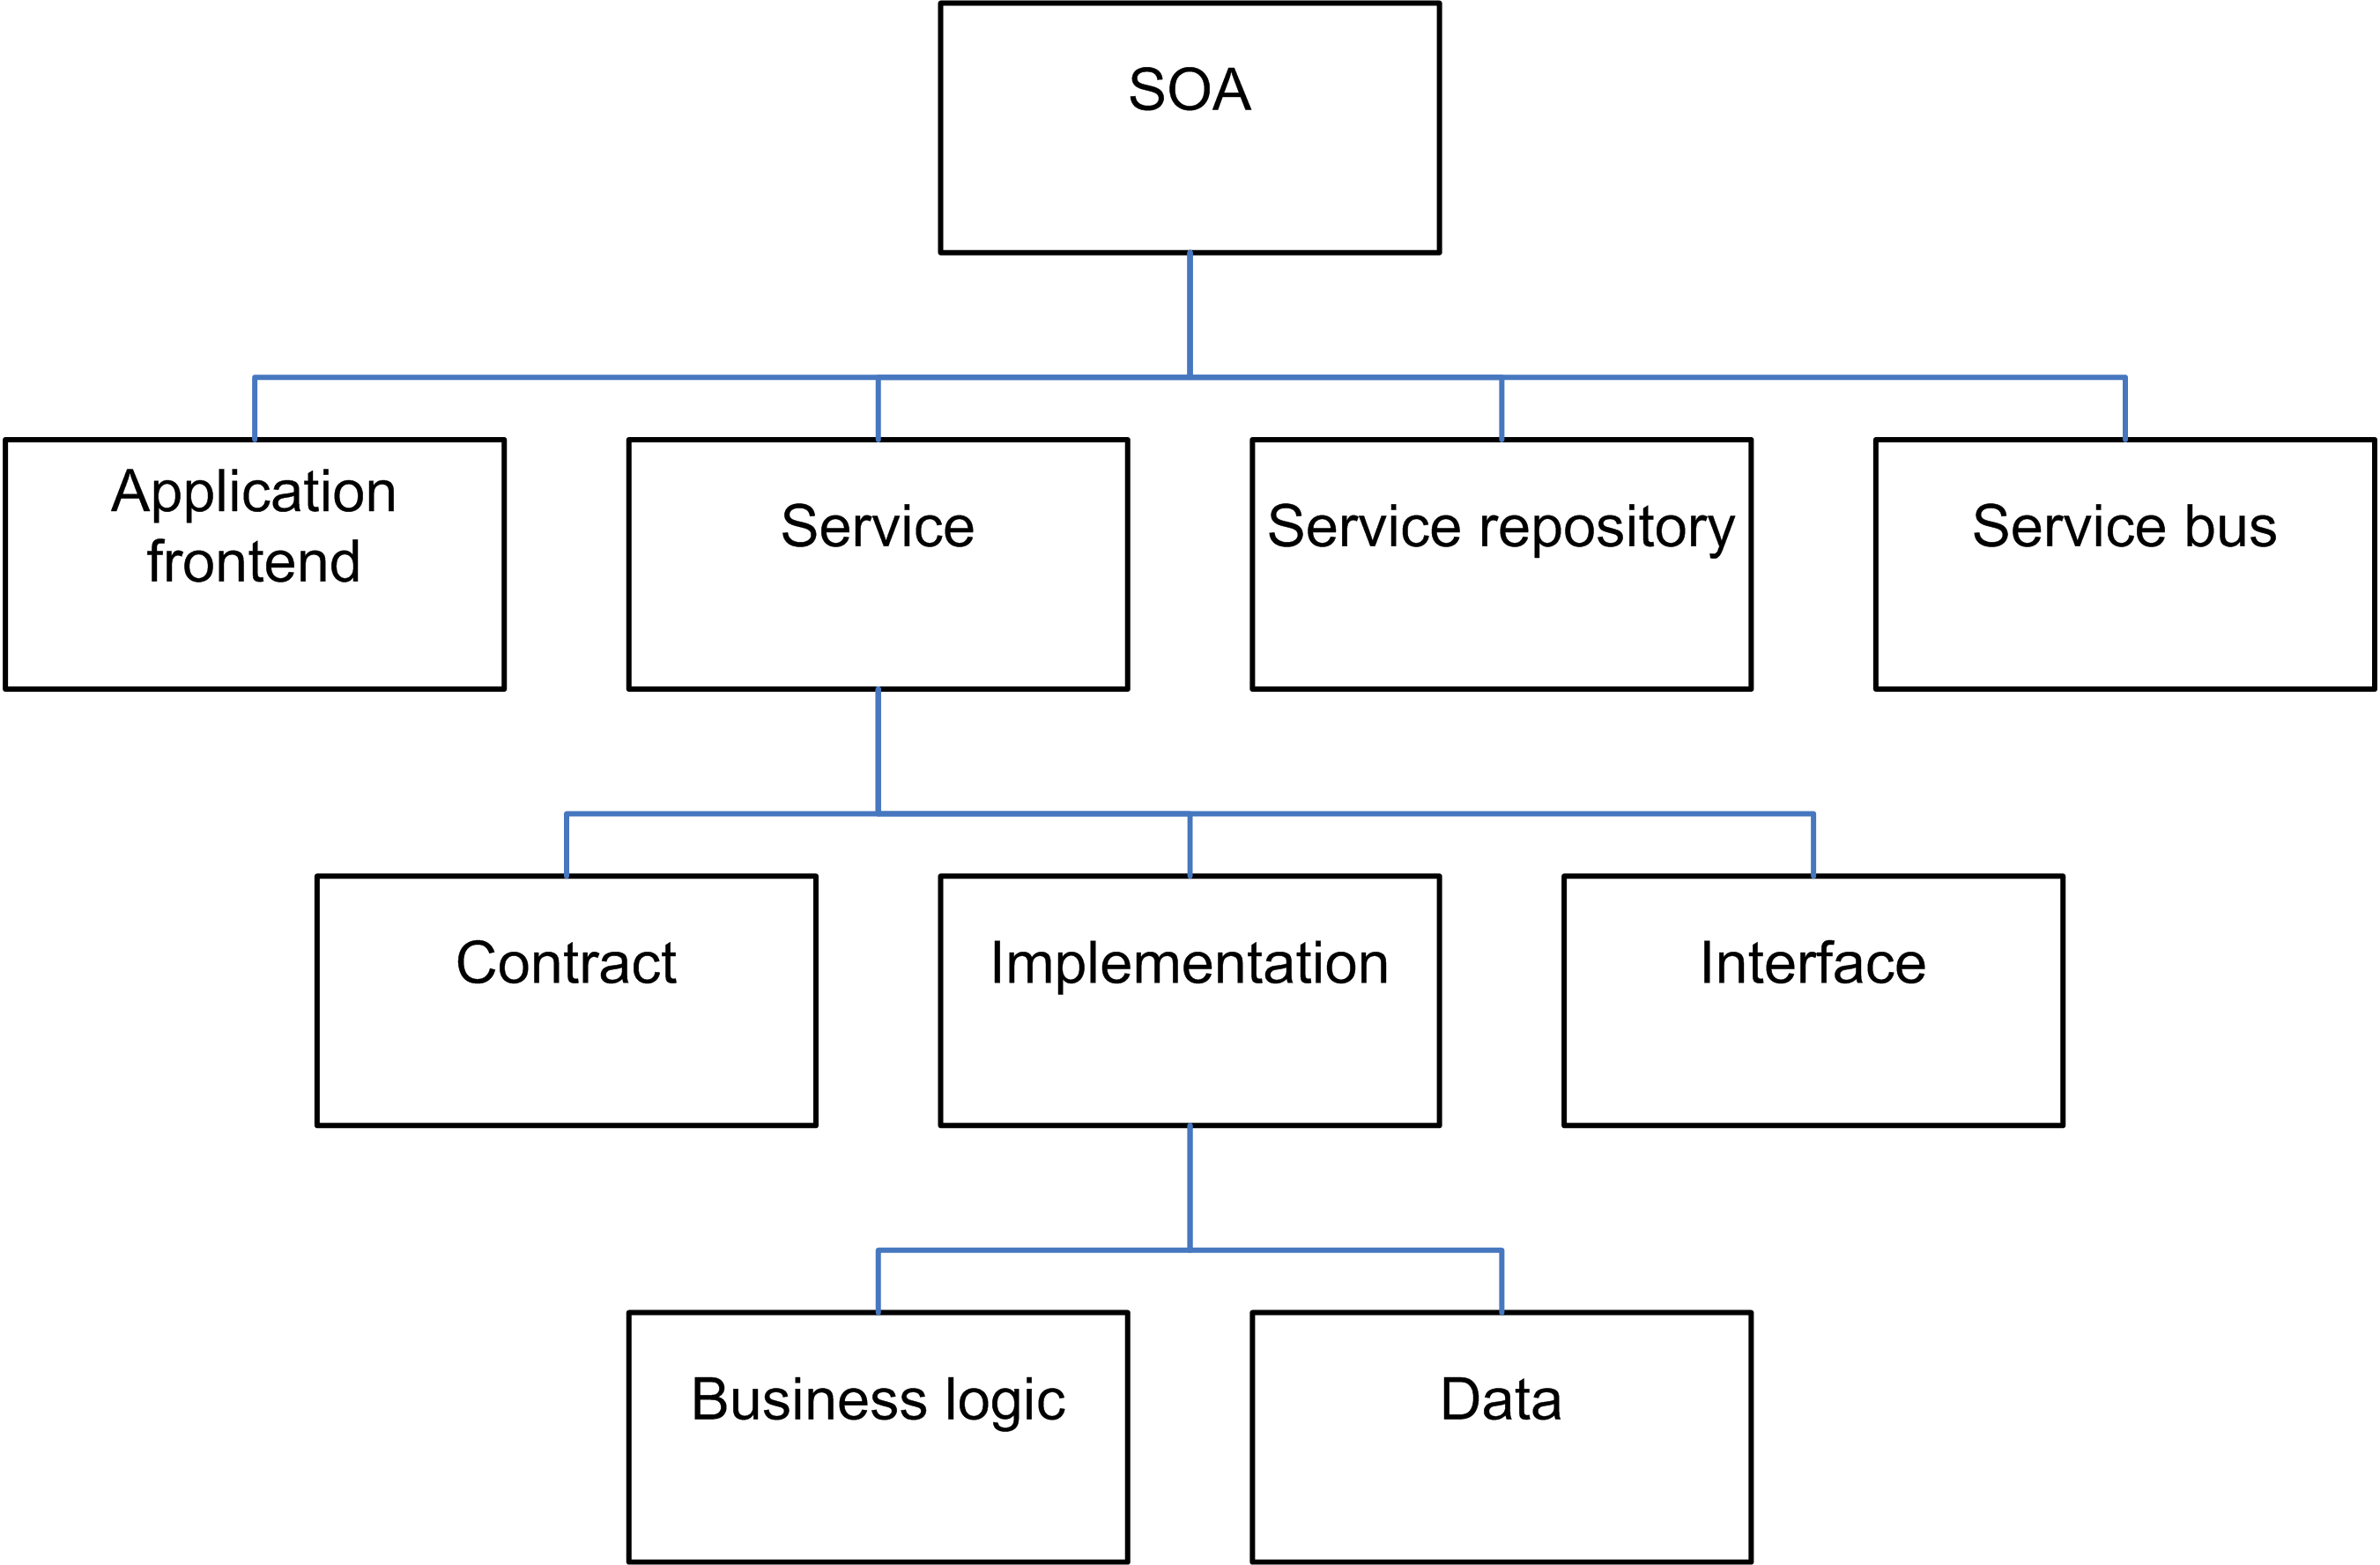
\includegraphics[scale=1]{soa.png}
\caption{SOA elements.}
\label{fig_soa}
\end{figure}
	


\section{Master-Slave}
The Master-Slave pattern is used in real-time systems in which guaranteed interaction response times are required. It is another fundamental architecture developers use. It is used when you have two or more processes that need to run simultaneously and continuously but at different rates. If these processes run in a single loop, severe timing issues can occur. These timing issues occur when one part of the loop takes longer to execute than expected. If this happens, the remaining sections in the loop get delayed. The Master-Slave pattern consists of multiple parallel loops. Each of the loops may execute tasks at different rates. Of these parallel loops, one loop acts as the master and the others act as slaves. The master loop controls all of the slave loops, and communicates with them using messaging architectures. \\\\\\\\


\begin{figure}[h]
\centering
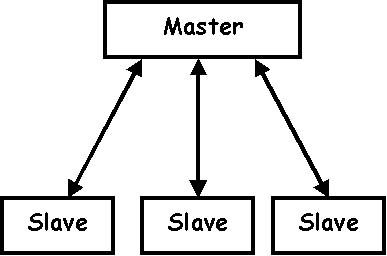
\includegraphics[scale=0.7]{ms.jpg}
\caption{Master-slave basic architecture.}
\label{fig_ms}
\end{figure}
\newpage




\newpage




\section{Message Bus}
A Message Bus is a combination of a common data model, a common command set, and a messaging infrastructure to allow different systems to communicate through a shared set of interfaces. This is analogous to a communications bus in a computer system, which serves as the focal point for communication between the CPU, main memory, and peripherals. Just as in the hardware analogy, there are a number of pieces that come together to form the message bus.\\\\\\


\begin{figure}[h]
\centering
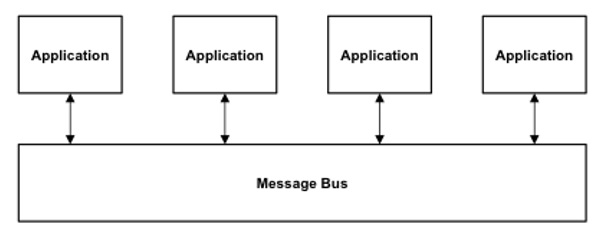
\includegraphics[scale=0.55]{mb.jpg}
\caption{Message bus architecture}
\label{fig_mb}
\end{figure}
\newpage



\section{Message Broker}
The Broker pattern is used to structure distributed systems with decoupled components, which interact by remote service invocations. Such systems are very inflexible when components have to know each others' location and other details (see Figure \ref{fig_mbr}). A broker component is responsible for the coordination of communication among components: it forwards requests and transmits results and exceptions. Servers publish their capabilities (services and characteristics) to a broker. Clients request a service from the broker, and the broker then redirects the client to a suitable service from its registry. Using the Broker pattern means that no other component than the broker needs to focus on low-level inter-process-communication.\\\\


\begin{figure}[h]
\centering
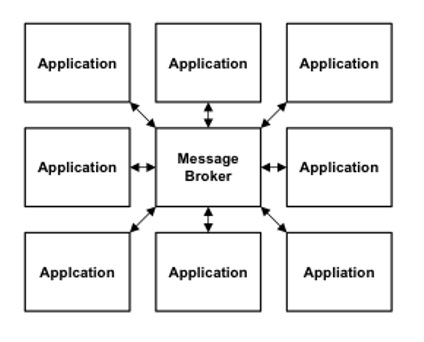
\includegraphics[scale=0.8]{mbr.jpg}
\caption{Message broker architecture}
\label{fig_mbr}
\end{figure}
\newpage



\section{Peer-to-peer}
The Peer-to-peer pattern can be seen as a symmetric Client-server pattern: peers may function both as a client, requesting services from other peers, and as a server, providing services to other peers. A peer may act as a client or as a server or as both, and it may change its role dynamically. Both clients and servers in the peer-to-peer pattern are typically multithreaded. The services may be implicit (for instance through the use of a connecting stream) instead of requested by invocation. Peers acting as a server may inform peers acting as a client of certain events. Multiple clients may have to be informed, for instance using an event-bus.\\\\



\begin{figure}[h]
\centering
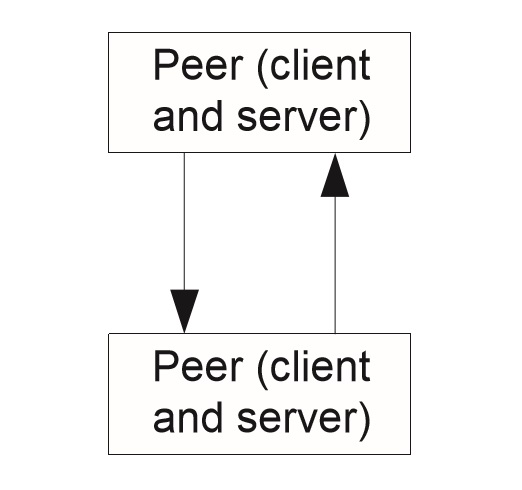
\includegraphics[scale=0.5]{p2p.jpg}
\caption{Peer-to-peer architecture}
\label{fig_mbr}
\end{figure}
\newpage



\section{Call and Return}
A call and return architecture enables software designers to achieve a program structure, which can be easily modified. This style consists of the following two substyles: \\

\begin{itemize}

\item \textbf{Main program/subprogram architecture} - In this, function is decomposed into a control hierarchy where the main program invokes a number of program components, which in turn may invoke other components.\\\\

\begin{figure}[h]
\centering
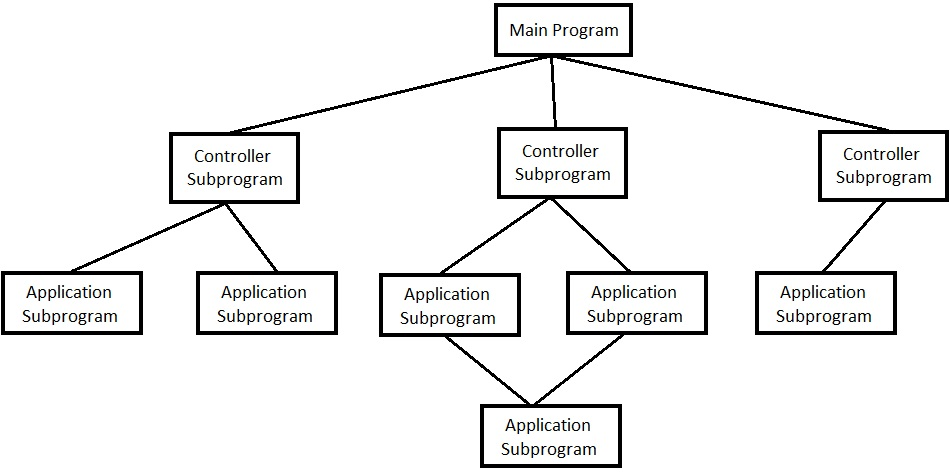
\includegraphics[scale=0.5]{c&r.jpg}
\caption{Main program/subprogram architecture}
\label{fig_c&r}
\end{figure}


\item \textbf{Remote procedure call architecture} - In this, components of the main or subprogram architecture are distributed over a network across multiple computers.

\end{itemize}
\newpage



\end{document}